\documentclass{beamer}
\usetheme[progressbar=foot, numbering=counter, block=fill]{metropolis}

\AtBeginSection[]
{
  \begin{frame}<beamer>
    \frametitle{Table of Contents}
    \tableofcontents[currentsection]
  \end{frame}
}

\title{Self-regulation and mathematics learning in the college classroom}
\date{October 30, 2018}
\author{Jenny Lee}
\institute{Harvey Mudd College\\Advisor: Dagan Karp}
\begin{document}
\maketitle
\begin{frame}{Recap \& Overview}

  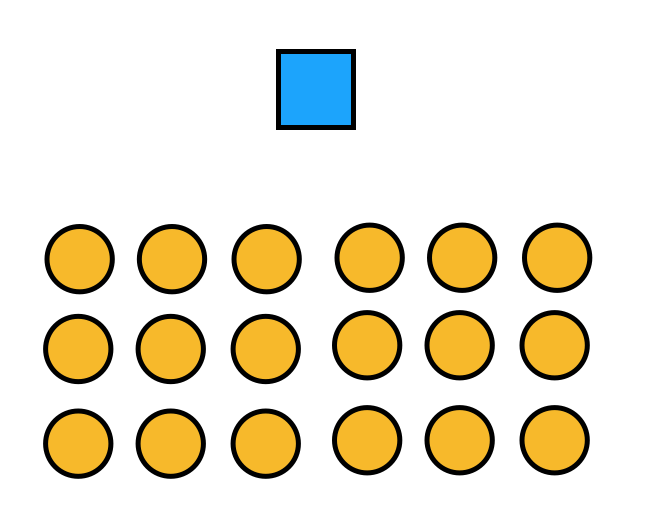
\includegraphics[width=5cm]{lecturestyle1}
  \hfill
  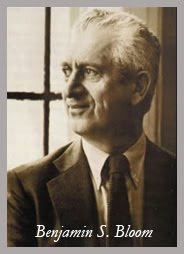
\includegraphics[width=4cm]{bloom.jpg}

  \begin{itemize}
    \item Context of fairness in mathematics
    \item Self regulation in action
    \item Case study
  \end{itemize}
\end{frame}
\begin{frame}{Mathematics is not fair.}
  \begin{itemize}
  \item Centralized locus of power\pause
  \item Generalized instruction, individualized assessment\pause
  \item A system built to benefit a specific subset of the population.
  \begin{itemize}
    \item Biases (instructional, structural)
    \item Cultural obstructions
  \end{itemize}
  \end{itemize}

      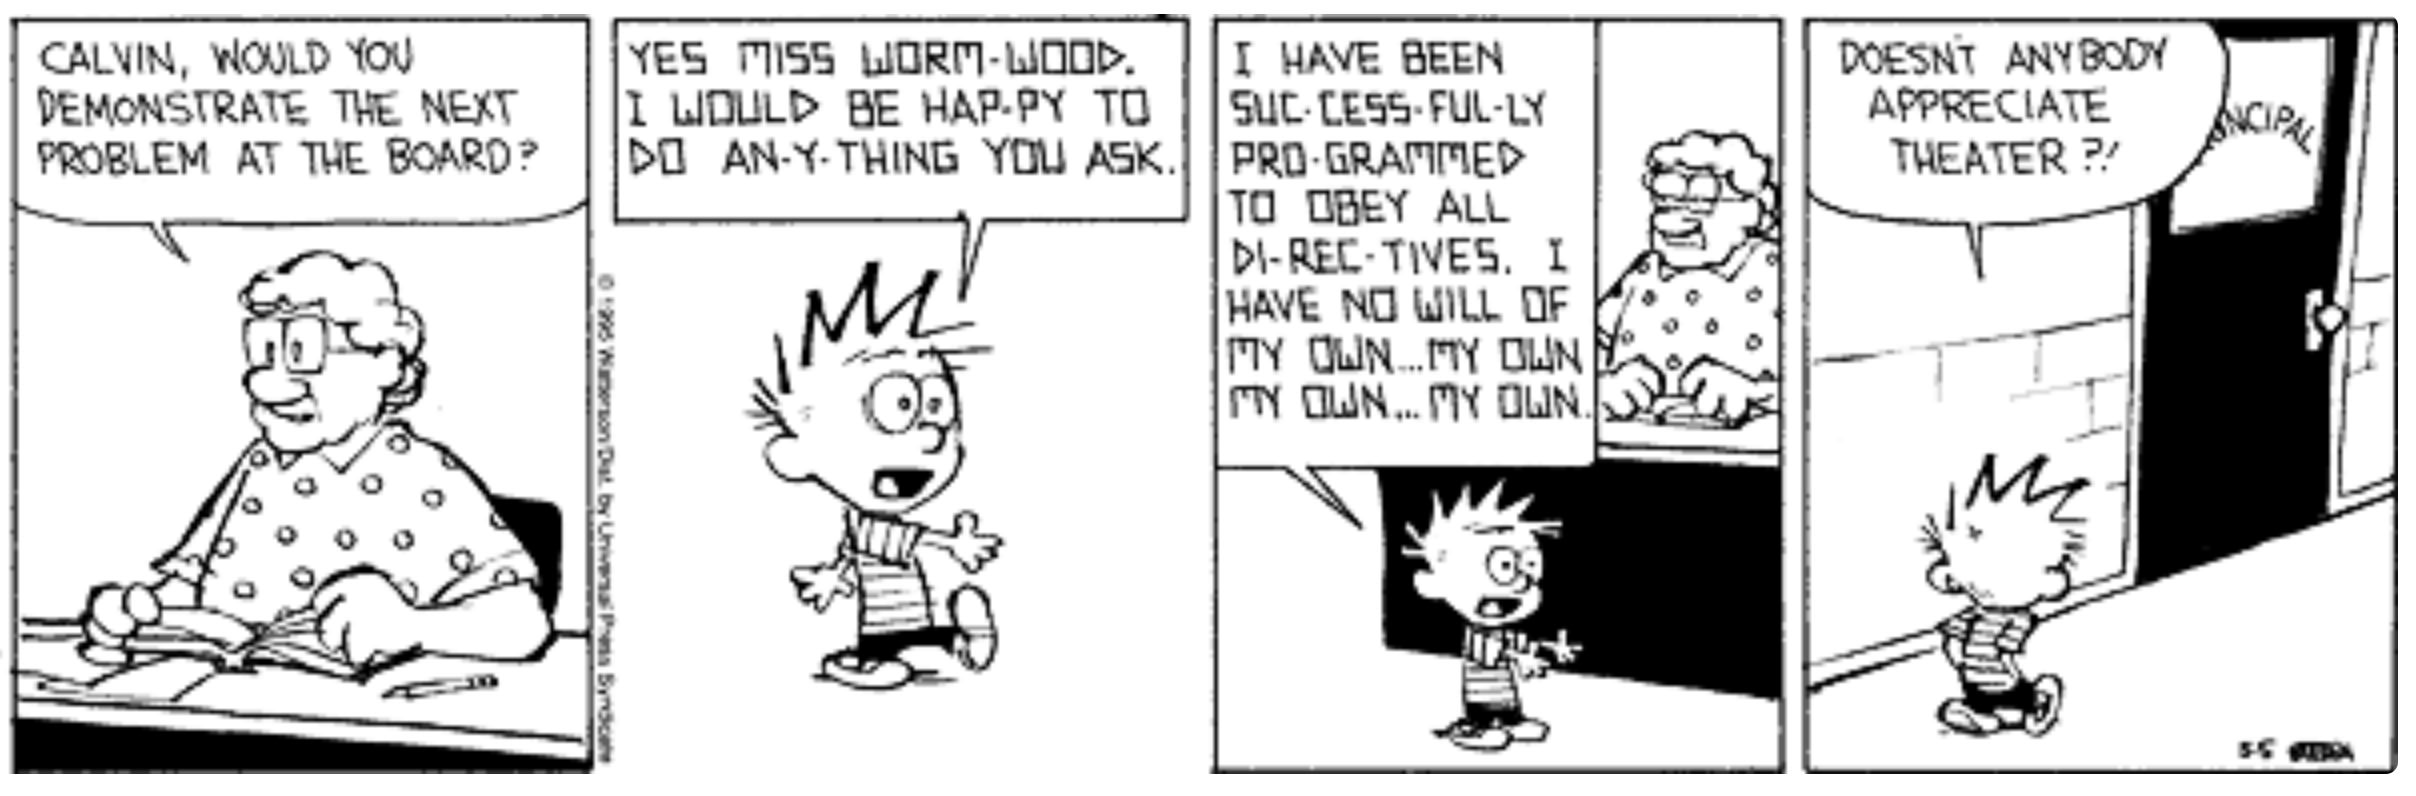
\includegraphics[width=\textwidth]{ch3}

\end{frame}
\begin{frame}{Cultural obstructions}

      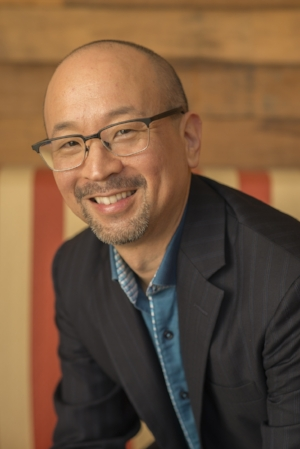
\includegraphics[width=3cm]{kumashiro}
      \hfill
      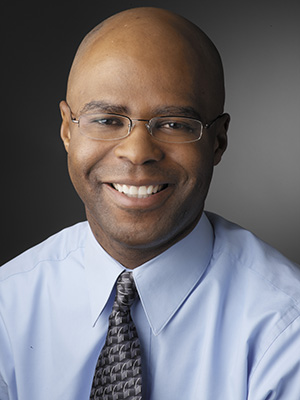
\includegraphics[width=3cm]{danny}
      \hfill
      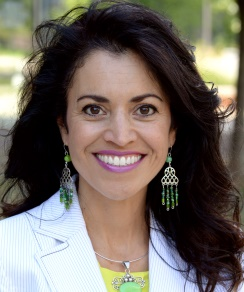
\includegraphics[width=3cm]{rochelle}

  \begin{itemize}
    \item Anti-oppressive education (Kevin Kumashiro)\pause
    \item Mathematics as a racial project (Danny Martin)\pause
    \item Rehumanizing and decolonizing mathematics (Rochelle Gutierrez)
  \end{itemize}
\end{frame}
\begin{frame}{Self-regulation}
  Definition:
  \begin{center}
    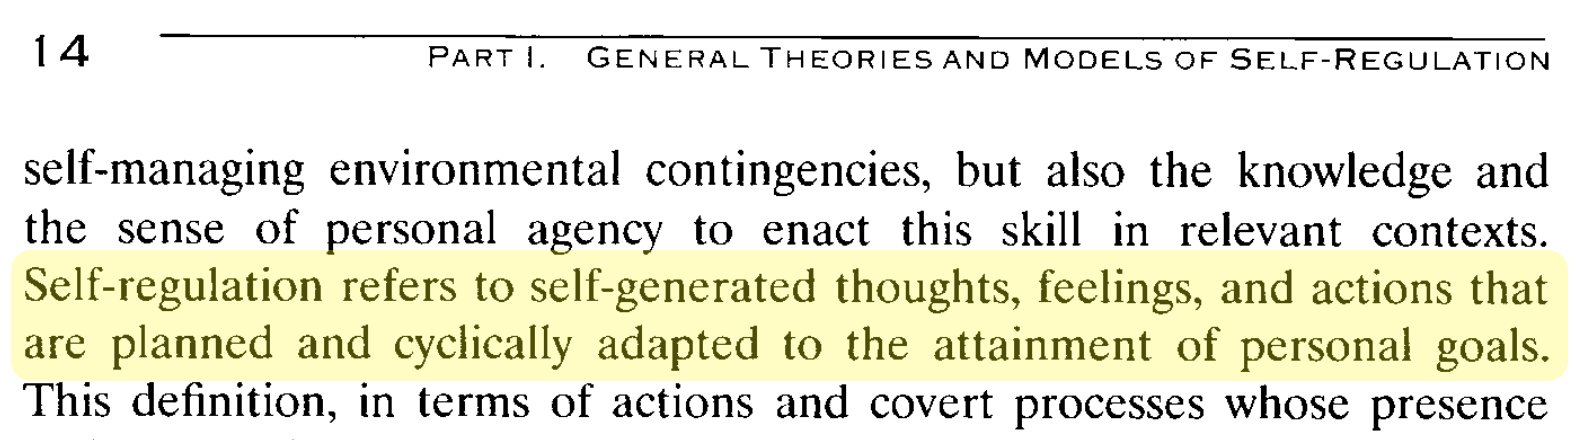
\includegraphics[scale=0.4]{selfregdef}
  \end{center}
  \hfill \begin{minipage}[]{7cm}
      \emph{\tiny Zeidner, M., Pintrich, P. R., \& Boekaerts, M. (2005). Handbook of Self-Regulation. Burlington, MA: Academic Press.}
\end{minipage}
\end{frame}
\begin{frame}{Self-regulation}
  \begin{itemize}
    \item Changing the perception of mathematics (imposed by self, not society)
    \item Effecting self-perception as a mathematician (self-efficacy)
    \item {\bf How can we use self-regulation to shift the locus of power?}
  \end{itemize}
\end{frame}
\begin{frame}{Self-regulation in the wild}
  \begin{itemize}
    \item Self-instruction
    \begin{itemize}
      \item Moore method
      \item ex. Flipped classrooms, inquiry-based learning
    \end{itemize}
    \item Self-monitoring
    \begin{itemize}
      \item Scheduling and planning ahead
      \item Immediate and private feedback via checklists
      \item Concrete and continuous understanding of own performance
    \end{itemize}
  \end{itemize}
\end{frame}
\begin{frame}{One form of self-regulation: self-assessment}
  \begin{itemize}
    \item Qualitative or quantitative evaluation, independently completed
    \item Practicing metacognitive skills as a part of the assessment (implicitly) \pause
    \item Goal: build independent thought, shift locus of power, move away from standardization
  \end{itemize}
\end{frame}
\begin{frame}{Case study: Math 40}

  
\includegraphics[width=\textwidth]{ch.jpg}

  \begin{itemize}
    \item Relatively ideal (school, size, subject)
    \item Implementation
    \begin{itemize}
      \item Students in section A - regular midterm/exam
      \item Students in section B - multiple take-home quizzes with multiple retries without penalty
    \end{itemize}
  \end{itemize}
\end{frame}
\begin{frame}{Results from the case study}
  \begin{itemize}
    \item ``No negatives'' = equally effective academic achievement
    \item Positive student experience
    \begin{itemize}
      \item Less stress
      \item ``Quizzes help break things up'', ``I can take my time'', ``Incentive to study''
    \end{itemize}
    \item Signs of self-regulation in action
    \begin{itemize}
      \item Using first quiz as learning tool
      \item Scheduling and/or asking for deadlines
      \item Setting a limit to retakes
    \end{itemize}
  \end{itemize}
\end{frame}
\begin{frame}{What this means}
  \begin{itemize}
    \item Speculative remarks
    \item A question to consider
  \end{itemize}
\end{frame}
\end{document}
